\chapter{Topologically protected MBQC}
\label{Chap:TMBQC}
In this chapter, 
we reformulate topological fault-tolerant quantum computation
explained in the previous chapter
in terms of meausrement-based quantum computation.

\section{Topological cluster state in 3D}
Consider a (primal) cubic lattice $\mathcal{L}$ 
and $\mathbf{Z}_2$ chain complex on it, $\{ C_0, C_1, C_2, C_3\}$,
where
\begin{eqnarray}
c_0 &=& \sum _k z_k v_k \in C_0, \;\;\;
c_1 = \sum _l z_l e_l \in C_1, 
\\
c_2 &=& \sum _m z_m f_m \in C_2, \;\;\;
c_3 = \sum _n z_n q_n \in C_3, \;\;\;
\end{eqnarray}
with $z_k,z_l, z_m, z_n \in \mathbf{Z}_2$.
We also consider a dual cubic lattice $\bar{\mathcal{L}}$
through the relations $v_k \leftrightarrow \bar q_k$,
$e_l \leftrightarrow \bar f_l$, $f_m \leftrightarrow \bar e_m$,
and $q_n \leftrightarrow \bar v_n$.

Qubits are defined on the edges and faces of the primal lattice $\mathcal{L}$ (or equivalently primal and dual edges), as shown in Fig.~\ref{figAp01}.
%%%%
\begin{figure}[t]
\centering
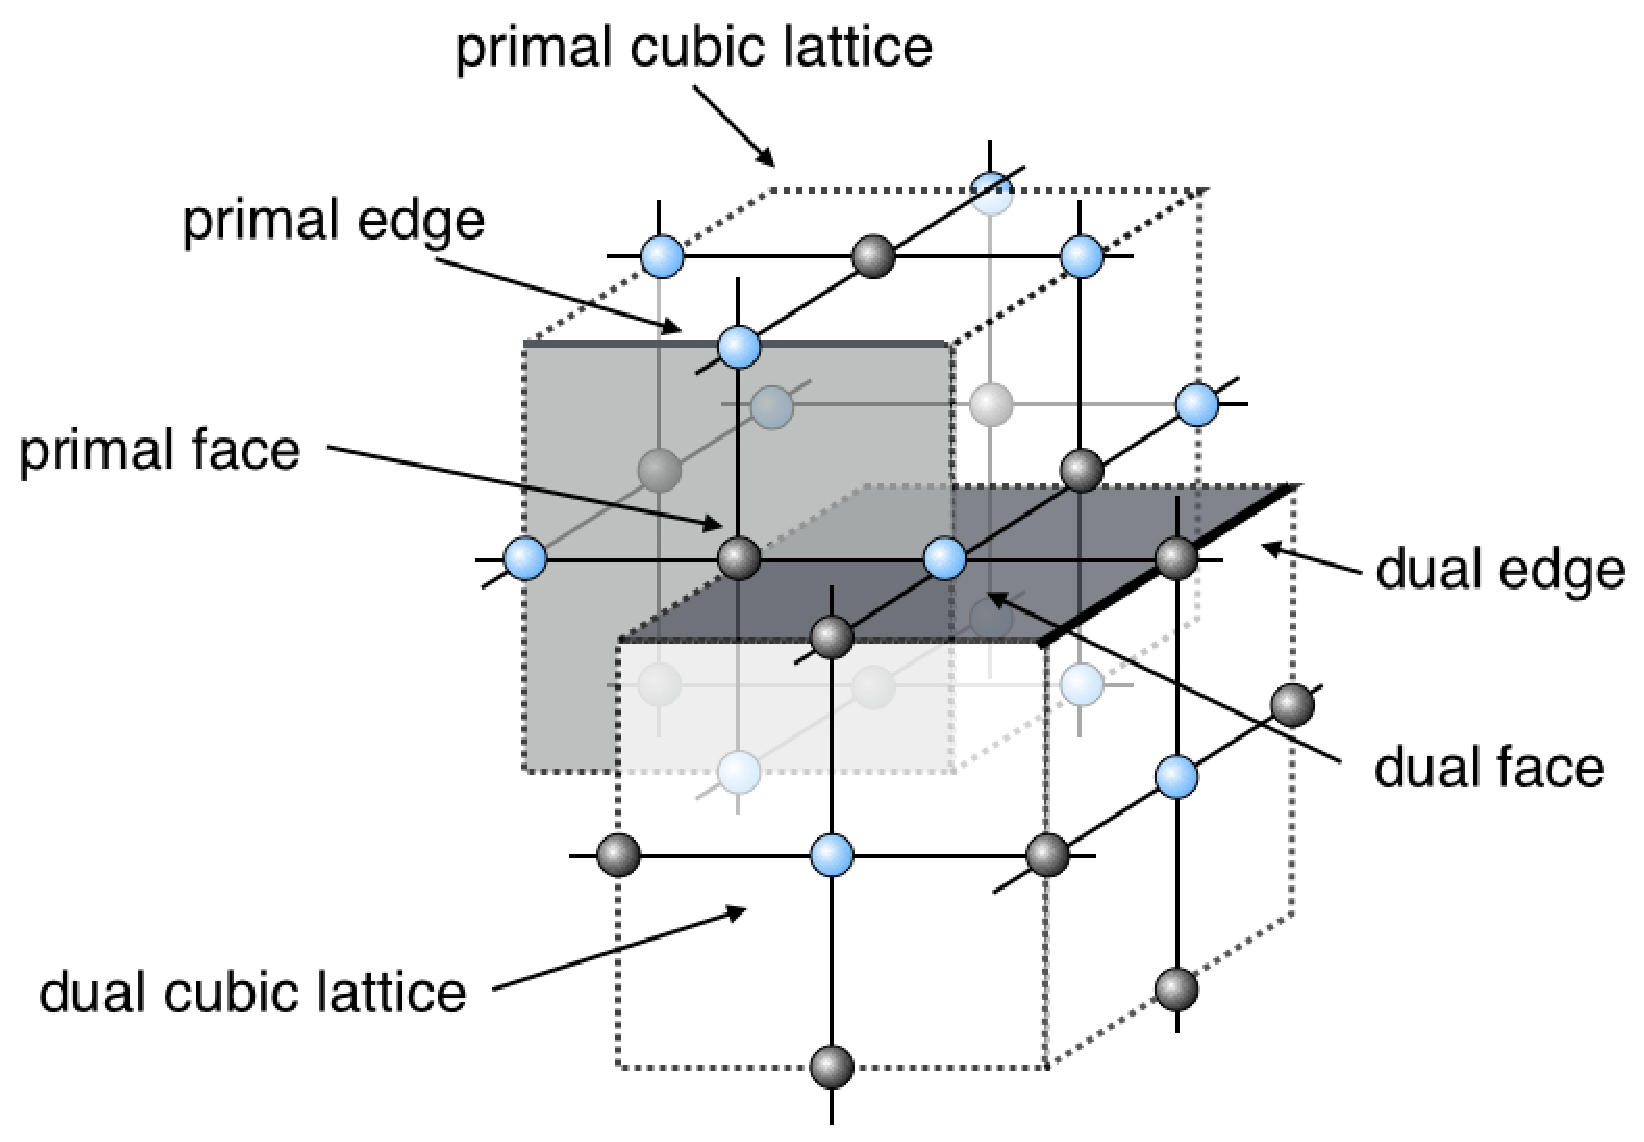
\includegraphics[width=120mm]{figAp01.eps}
\caption{A unit cell of the cluster state for topological MBQC. 
The primal and dual cubes, faces, and edges are also shown.
}
\label{figAp01}
\end{figure}
%%%%
We define an operator $A(c_i)$ ($i=1,2$) 
in terms of a 1-chain $c_1 = \sum _j z_j e_j$ or a 2-chain $c_2=\sum _j z_j f_j$
as 
\begin{eqnarray}
A(c_i) = \prod _{j} A^{z_j}.
\end{eqnarray}
The stabilizer generators of a 3D cluster state for topologically protected MBQC are defined on the primal and dual elementary faces $f_m$, $\bar f_{m'}$ (see Fig.~\ref{figAp02} (a)): 
\begin{eqnarray}
K_{f_m} &=& X_{f_m} Z(\partial f_m),
\\
K_{\bar f_{m'}} &=& X_{\bar f _ {m'}} Z(\partial \bar f_{m'}).
\end{eqnarray}
%%%%
\begin{figure}[t]
\centering
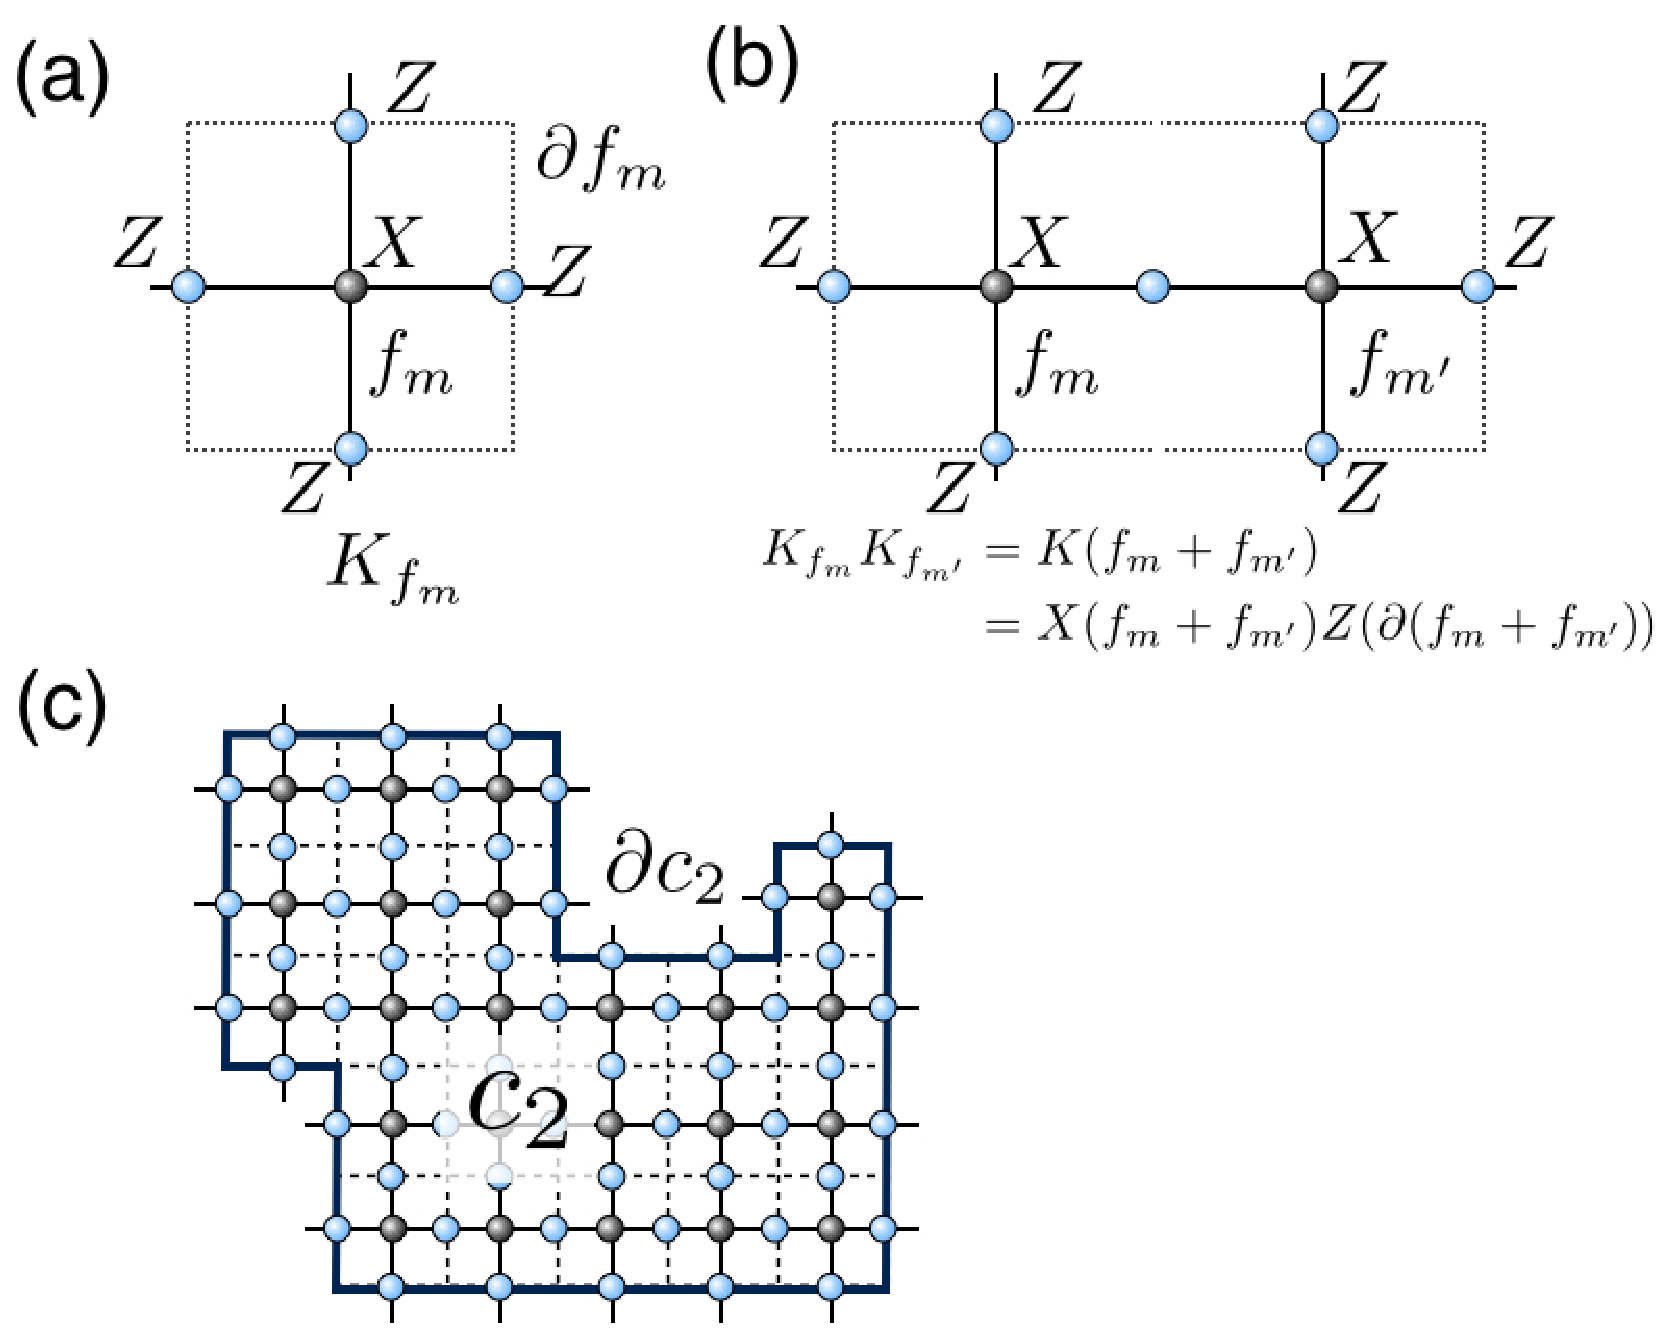
\includegraphics[width=120mm]{figAp02.eps}
\caption{(a) A stabilizer operator defined on a primal face.
(b) $K_{f_m} K_{f_{m'}} = X(f_m+f_{m'}) Z(\partial (f_m+f_{m'}))$. 
(c) $K(c_2) \equiv \prod _m K_{f_m}^{z_m} = X(c_2) Z(\partial c_2)$.}
\label{figAp02}
\end{figure}
%%%%
A unit cell of the 3D cluster state is shown in Fig.~\ref{figAp01}.
This notion of stabilizer generators of the cluster state is quite useful; it provides a connection between the operators and the chain complex as follows.
By multiplying the two stabilizer operators $K_{f_m}$ and $K_{f_{m'}}$, we have 
\begin{eqnarray}
K_{f_m} K_{f_{m'}} = X(f_m+f_{m'}) Z(\partial (f_m+f_{m'})),
\end{eqnarray}
(see also Fig.~\ref{figAp02} (b)).
By using this property, we can define a stabilizer operator on a 2-chain $c_2$,
\begin{eqnarray}
K(c_2) \equiv \prod _m K_{f_m}^{z_m} = X(c_2) Z(\partial c_2),
\end{eqnarray}
(see also Fig.~\ref{figAp02} (c)).
Furthermore, for the two 2-chains, $c_2$ and $c'_2$, we have
\begin{eqnarray}
K(c_2+c'_2)= K(c_2)K(c'_2).
\end{eqnarray}

Let us see how the 3D cluster state is related to 
topological quantum computation on the surface code 
explained in Chapter~\ref{Chap:TQC}.
Recall the circuit diagrams for the 
syndrome measurements of the plaqette and star operators
in Fig.~\ref{fig83}.
The measurement for the plaquette operator is done by 
applying the CZ gates between 
the ancilla qubit on the face center and the four qubits on the edges.
This operation is the same as generation of the cluster state
stabilized by $K(f_m)$ with a horizontal face $f_m$.
The syndrome measurement for the star operator 
can be done by the CZ gates with the basis change by 
the Hadamard gates.
This corresponds to generation of the cluster state
stabilized by $K(\bar f_l)$ with a horizontal dual face $\bar f_l$.
Moreover, the horizontal edge qubits,
which constitute the surface code, are connected 
by applying the CZ gates vertically
in order to perform the Hadamard gates for the basis change.
In this way, we recover the 3D cluster state
stabilized by $K(f_m)$ and $K(\bar f_l)$
for all primal and dual faces $f_m$ and $\bar f_l$.
Two of three dimensions are employed for the 
spatial degrees of freedom, constituting the surface code.
One is for the time evolution of measurement-based quantum computation.
The measurements are done along the time-like axis,
where even and odd layers,
corresponding to the syndrome measurements 
of the plaquette and star operators respectively, 
together with constitute an elementary time step of the topologically 
protected MBQC.
Below we will see how the topological operations on 
the surface code are translated into a measurement pattern 
of the MBQC on the 3D cluster state.

\section{Vacuum, defect, and singular qubit regions}
The cubic lattice is divided into three regions: the vacuum $\mathcal{V}$, defect $\mathcal{D}$, and singular qubits $\mathcal{S}$ (the detailed definitions are provided later).
In the vacuum region, the topological quantum computation is protected
through topological quantum error correction.
The defect regions are utilized to implement topological quantum computation by braiding defects. 
We have two types of defects: the primal ($D$) and dual ($\bar D$) defects.
For simplicity, we only consider the primal defect.
The extension to the dual case is straightforward by replacing primal by dual in the derivation.
The primal defect $D$ is defined as a set of primal cubes.
The primal face qubits inside the primal defect (except for those on the boundary $\partial D$) are measured in the $Z$-basis to remove the corresponding bonds of the cluster state (or, equivalently, we can prepare the cluster state without those bonds from the beginning).
On the boundary $\partial D$, the primal face qubits are measured in the $X$-basis.
The primal edge qubits belonging to the primal defect (including its boundary) are measured in the $X$-basis.
The measurement pattern for the dual defect is defined similarly.

Unfortunately, only Clifford circuits such as Pauli-basis preparations, measurements, and CNOT gates, are implemented in a topologically protected way.
For universal quantum computation, magic states for the non-Clifford gates are injected on the singular qubits, 
which are always located in-between two defects.
The injections are executed by
measuring the singular qubits in the $Y$- and $(X+Y)/\sqrt{2}$-bases.
These measurements correspond to injections of $(|0\rangle + e^{-i\pi/2}|1\rangle)/\sqrt{2}$ and $(|0\rangle + e^{-i \pi /4 }|1\rangle)/\sqrt{2}$ (up to global phases), 
which are utilized to implement the 
$S=e^{-i (\pi/4) Z}$ and $T= e^{-i (\pi /8) Z}$ gates via gate teleportation,
respectively.
The singular qubits are not topologically protected,
because two defects are made close to each other 
resulting in shortening the code distance.
However, we can obtain clean magic states 
with topologically protected Clifford gates through 
the magic state distillation protocols~\cite{Magic}.
In this way, an arbitrary quantum computation is executed fault-tolerantly.
Below, we will define these three regions more precisely 
and see how topological quantum computation 
is executed in a measurement-based way.



%%%%
\begin{figure}[t]
\centering
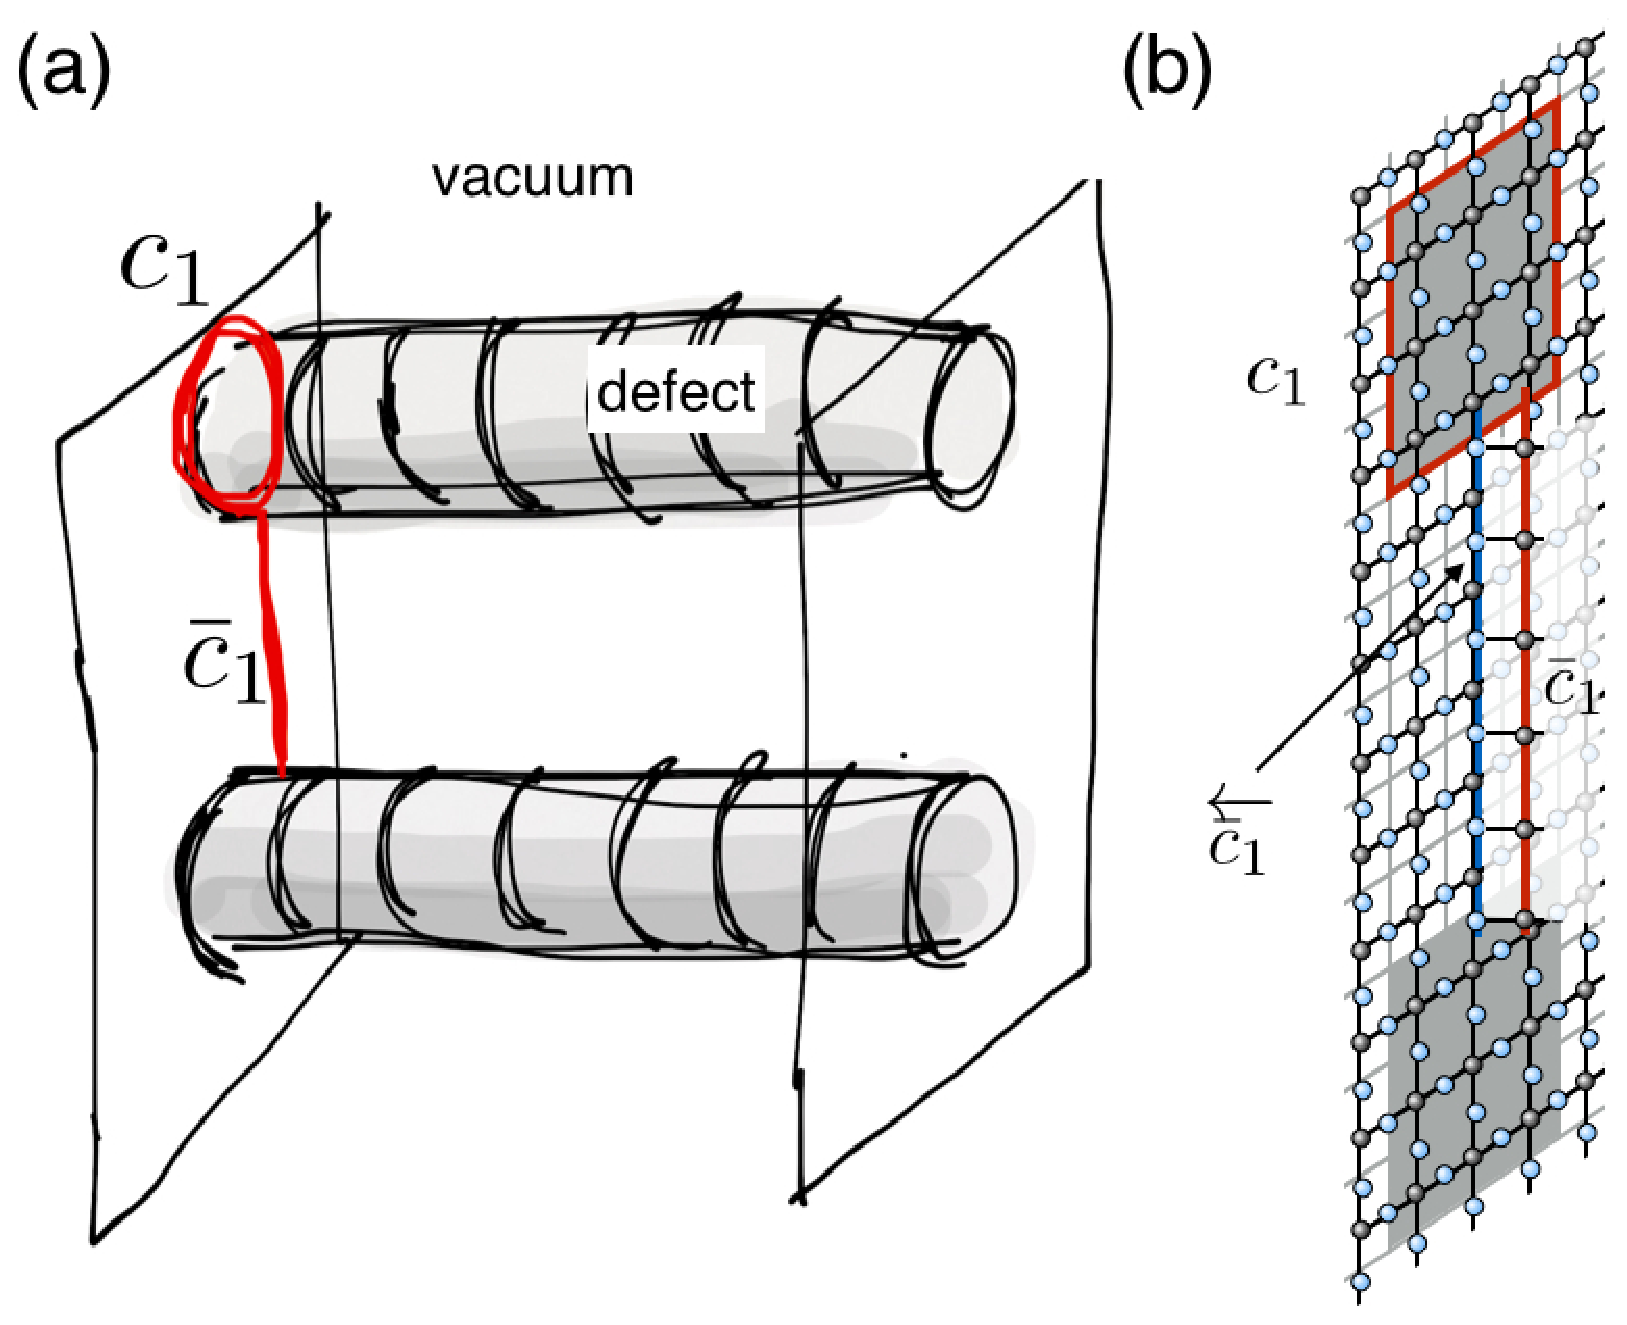
\includegraphics[width=80mm]{figAp03.eps}
\caption{(a) A defect pair logical qubit. 
(b) The logical operators $L_Z^{(t)}$ and $L_X^{(t)}$ at time step $t$.}
\label{figAp03}
\end{figure}
%%%%
\section{Elementary operations in topological MBQC}
\subsection*{Definition of a logical qubit}
The logical information is encoded by using a pair of two defects as shown in Fig.~\ref{figAp03} (a) and (b),
where the measurements are done from left to right.
The logical degree of information at time step $t$ is described a primal 1-chain $c_1$surrounding the defect and a dual 1-chain $\bar c_1$ connecting the two defects, as shown in Fig.~\ref{figAp03} (a).
After measuring qubits up to the $(t-1)$th even and odd layers, according to the measurement patterns presented before, the following two operators may become logical operators, which commute with the stabilizer group of the remaining cluster state and are independent of it:
\begin{eqnarray}
L^{(t)}_Z= Z(c_1), \;\;\; L^{(t)}_X= X(\overleftarrow {\bar c_1}) Z(\bar c_1),
\label{eq:cluster_logical}
\end{eqnarray}
where $\overleftarrow{\bar c_1}$ indicates the dual face qubits on the even layer at time step $t$ 
that are the left neighbor of $\bar c_1$ , as shown in Fig.~\ref{figAp03} (b).
These two operators anticommute with each other and represent a logical qubit.
(If the cluster state ends at the even layer at the time step $t$, then the two logical operators are equivalent to the logical operators of the surface code.
Because there are the time-like CZ gates for the Hadamard gates,
the logical $X$ operator in Eq. (\ref{eq:cluster_logical}) accompanied
by the $Z$ operators.)

%%%%
\begin{figure}[t]
\centering
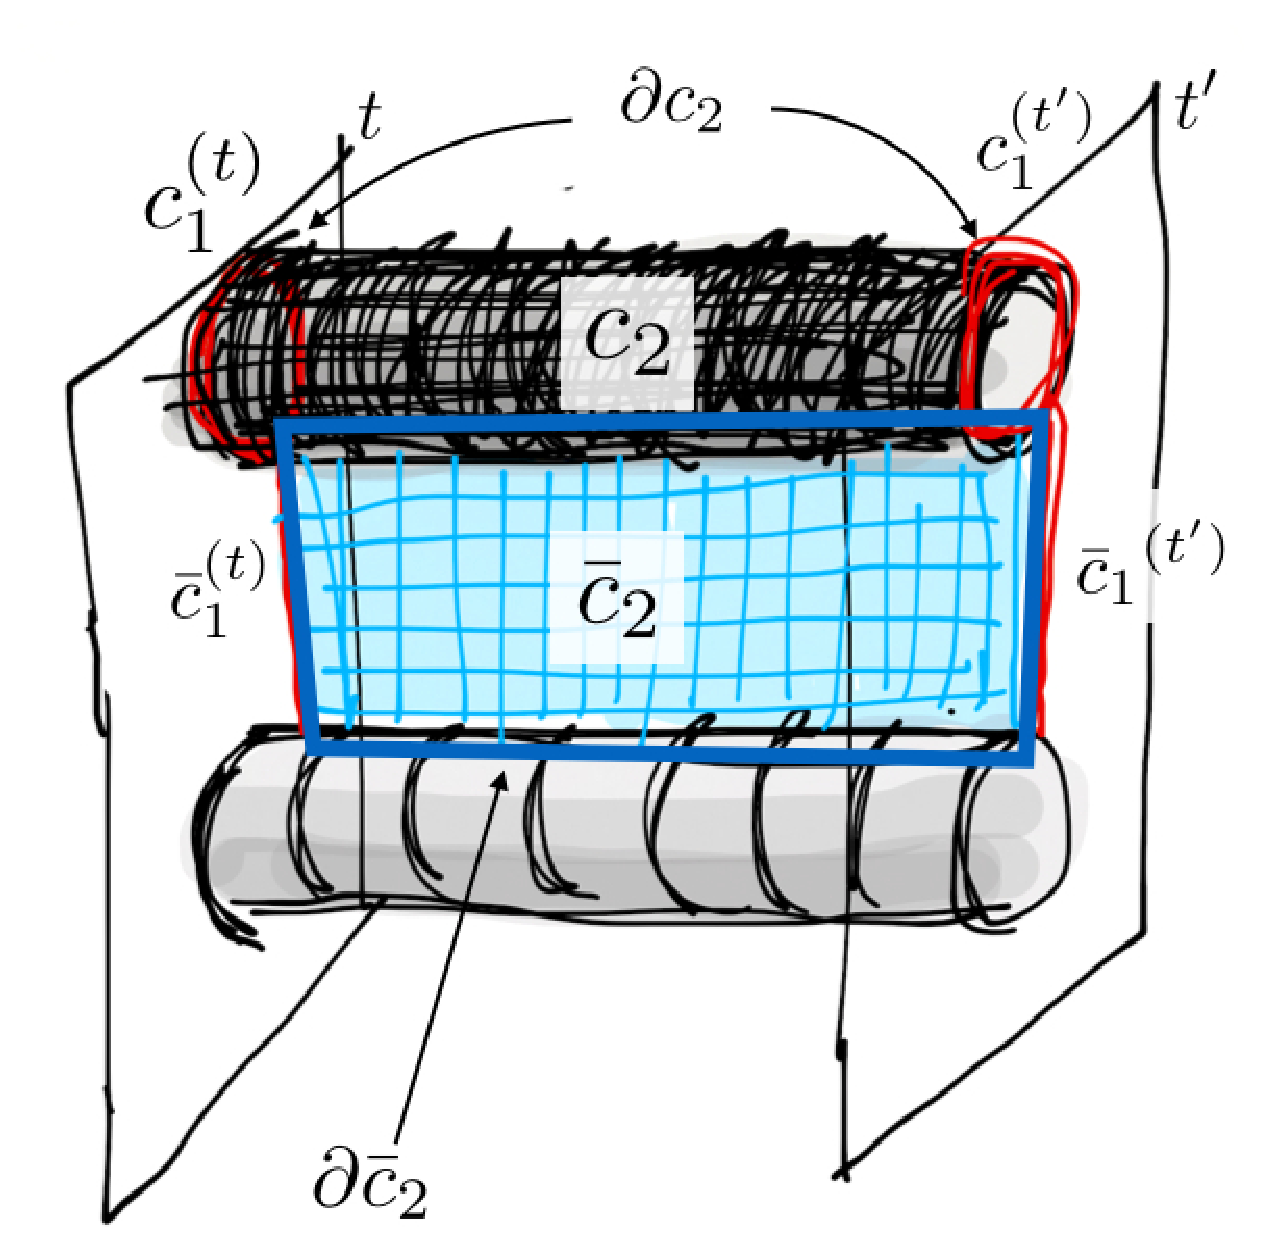
\includegraphics[width=80mm]{figAp04.eps}
\caption{A logical identity gate. 
The logical operators at time steps $t$ and $t'$ are related by the correlation surfaces $K(c_2)$ and $K(\bar c_2)$ via the measurements.
}
\label{figAp04}
\end{figure}
%%%%
\subsection*{Identity gate}
Next, we will see how these logical operators evolve with the measurements.
We consider a correlation surface defined by a primal 2-chain $c_2$ and a dual 2-chain $\bar c_2$ as shown in Fig.~\ref{figAp04}.
A stabilizer operator $K(c_2)$ on the correlation surface $c_2$ surrounding the defect is obtained by multiplying the stabilizer generators $K_{f_m}$ on the primal 2-chain $c_2$:
\begin{eqnarray}
K(c_2 ) \equiv \prod _{m} K_{ f_m}^{z_m} = Z(\partial c_2) X(c_2).
\end{eqnarray}
Similarly, a stabilizer operator on the dual correlation surface $\bar c_2$ is defined by multiplying $K_{\bar f_m}$ on the dual 2-chain $\bar c_2$:
\begin{eqnarray}
K(\bar c_2 ) \equiv \prod _{m} K_{\bar f_m}^{z_m} = Z(\partial \bar c_2) X(\bar c_2).
\end{eqnarray}
%Because the even layer at the right end divides the dual faces in half,
%$Z(\overleftarrow{\bar c_1^{(t-1)}})$ is multiplied
%to cancel the boundary $Z$ operators at the right end, 
Suppose measurements are done from the left to the right, except for those qubits on the final even layer.
Using the correlation surface, we obtain equivalence relations between the logical operators at time $t$ and $t'$:
\begin{eqnarray}
L_Z^{(t)} &\sim& Z(c_1^{(t)}) K(c_2 ) = Z(c_1^{(t')}) X(c_2).
\\
L_X^{(t)} &\sim& X(\overleftarrow {\bar c^{(t)}_1}) Z(\bar c^{(t)}_1) K(\bar c_2) = X(\overleftarrow {\bar c_1}) X(\bar c_2) Z(\bar c^{(t')}_1) 
\end{eqnarray}
Here, $ A\sim B$ means that $A$ and $B$ are equivalent up to a multiplication of the stabilizer operator of the cluster state, meaning that both $A$ and $B$ act the same on the cluster state.
When the qubits on $c_2$ have been measured in the $X$-basis, we obtain 
\begin{eqnarray}
L_Z^{(t)} &\sim& L_Z^{(t+1)},
\\
L_X^{(t)} &\sim& L_X^{(t+1)},
\end{eqnarray}
where we assumed that all measurement outcomes are $+1$ for simplicity.
This relation indicates that the logical information at time step $t$ is propagated to time step $t'$ without any operation, i.e., a logical identity operation.

%%%%
\begin{figure}[t]
\centering
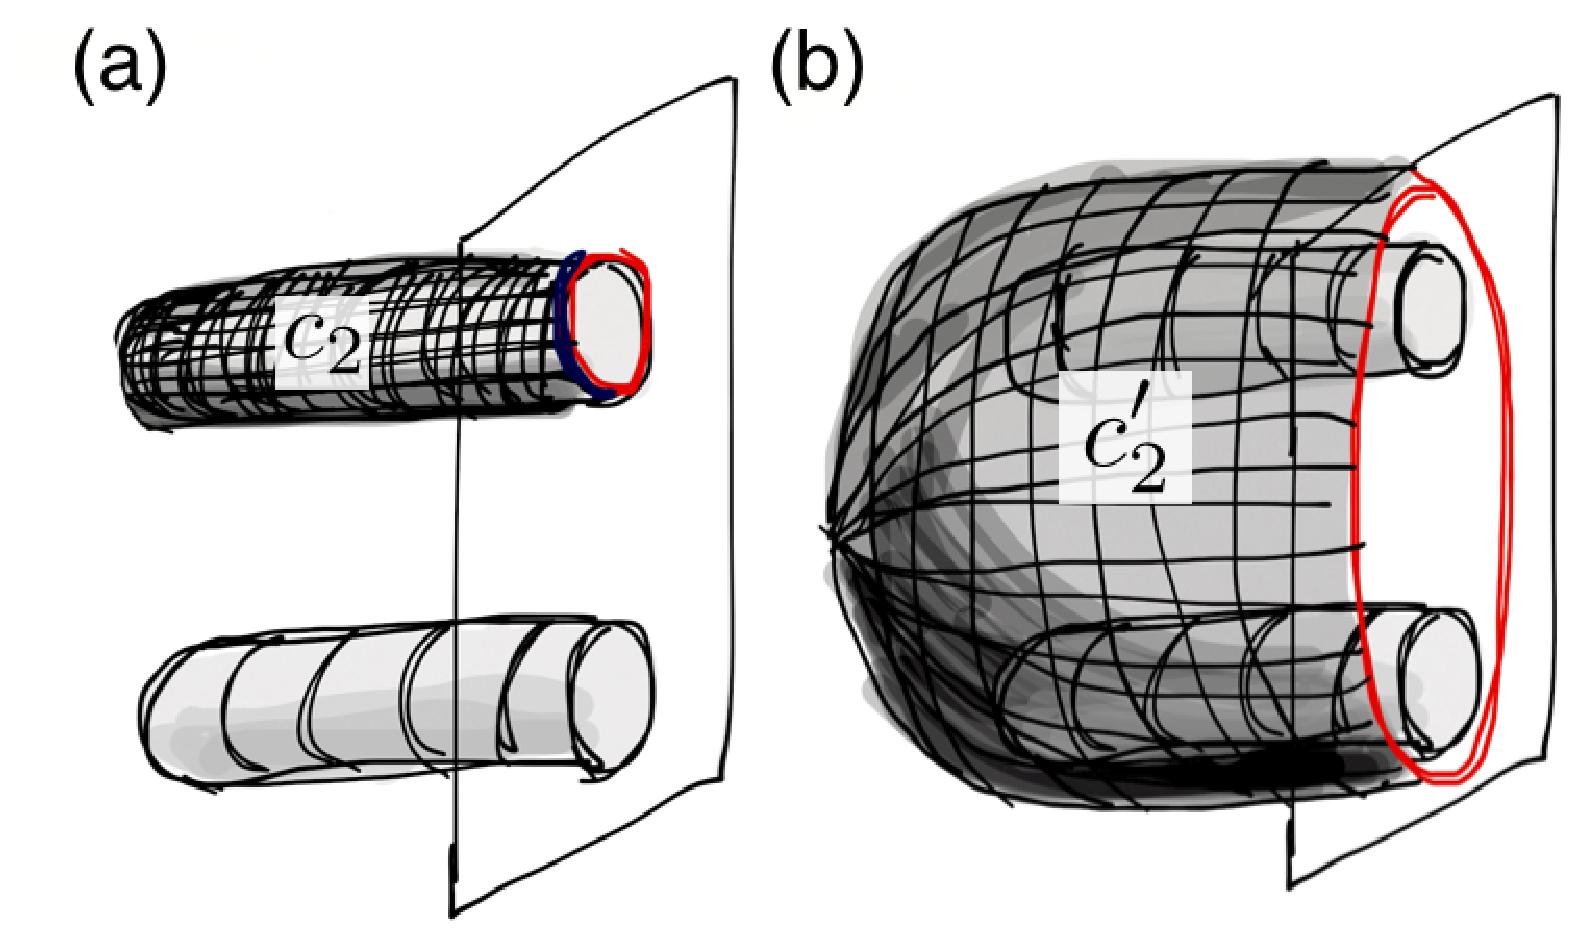
\includegraphics[width=80mm]{figAp05.eps}
\caption{(a) A logical $Z$-basis state preparation. 
(b) $K(c'_2)= X(c'_2) L_Z^{(t)} {L'_Z}^{(t)}$}
\label{figAp05}
\end{figure}
%%%%
\subsection*{State preparation and measurement}
Next, we consider how the logical qubit is prepared from the vacuum.
To prepare the eigenstate of $L_Z^{(t)}$, we utilize the defect shown in Fig.~\ref{figAp05} (a).
By considering the correlation surface $c_2$, we obtain
\begin{eqnarray}
K(c_2) = X(c_2) L_Z^{(t)}.
\end{eqnarray}
Because $X(c_2)$ commutes with the measurements, the state at time step $t$ is stabilized by $L_Z^{(t)}$, and hence a logical $Z$-basis state is prepared.
Considering another surface $c'_2$, shown in Fig.~\ref{figAp05} (b), the state at time step $t$ is also stabilized by $Z(\partial c'_2)=L_Z^{(t)} {L'_Z}^{(t)}$.
Thus the pair of the defects is appropriately encoded into the code space.
Both $L_Z^{(t)}$ and ${L'_Z}^{(t)}$ act equivalently as logical $Z$ operators.

%%%%
\begin{figure}[t]
\centering
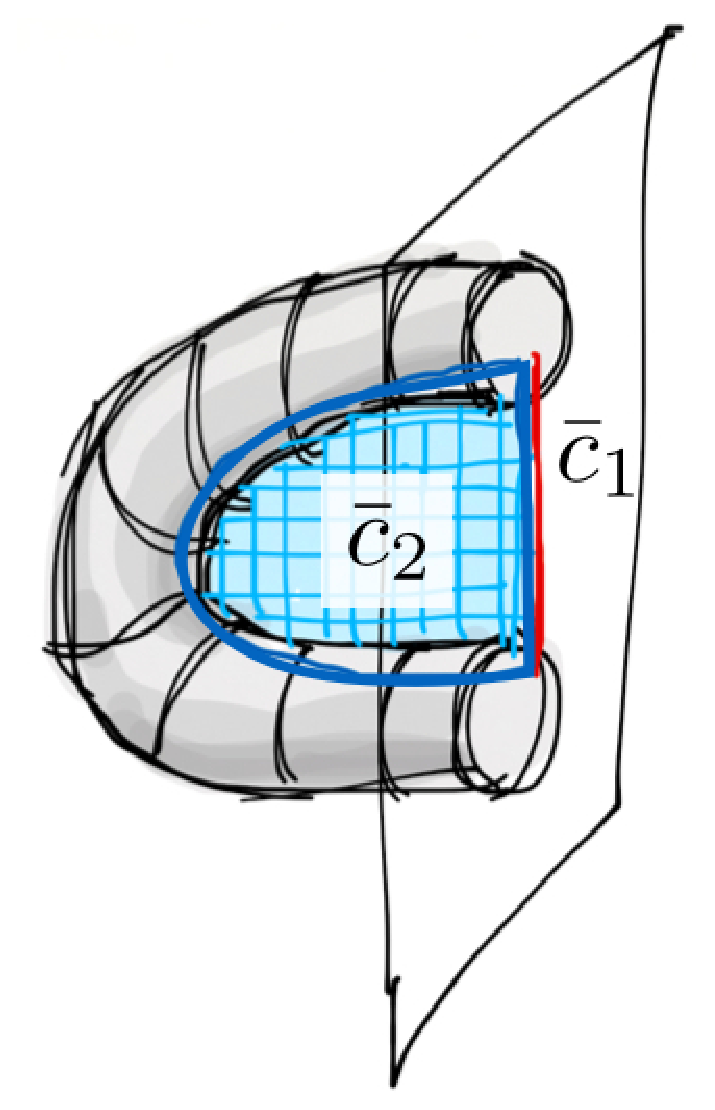
\includegraphics[width=55mm]{figAp06.eps}
\caption{A logical $X$-basis state preparation.}
\label{figAp06}
\end{figure}
%%%%
Next, we consider the defect shown in Fig.~\ref{figAp06}.
Considering a correlation surface $\bar c_2$, we obtain
\begin{eqnarray}
K(\bar c_2) = Z(\partial \bar c_2) X(\bar c_2).
\end{eqnarray}
After the measurements, the state at time step $t$ is stabilized by $L_X^{(t)}= X(\overleftarrow{\bar c_1}) Z(c_1)$, where $c_1$ is a 1-chain on the $t$th even layer connecting the two defects.
Thus, a logical $X$-basis state is prepared.
Again, the logical state is stabilized by $Z(c_1)Z(c'_1)$, with $c_1$ and $c'_1$ being a cycle surrounding each defect.
Hence, we can choose either $L_Z^{(t)}=Z(c_1)$ or $L_Z^{(t')}=Z(c'_1)$ to serve as the logical operator.
The logical measurements of the defect pair qubits can be done with the same defects as the state preparations, but by reversing the time-like direction.

%%%%
\begin{figure*}
\centering
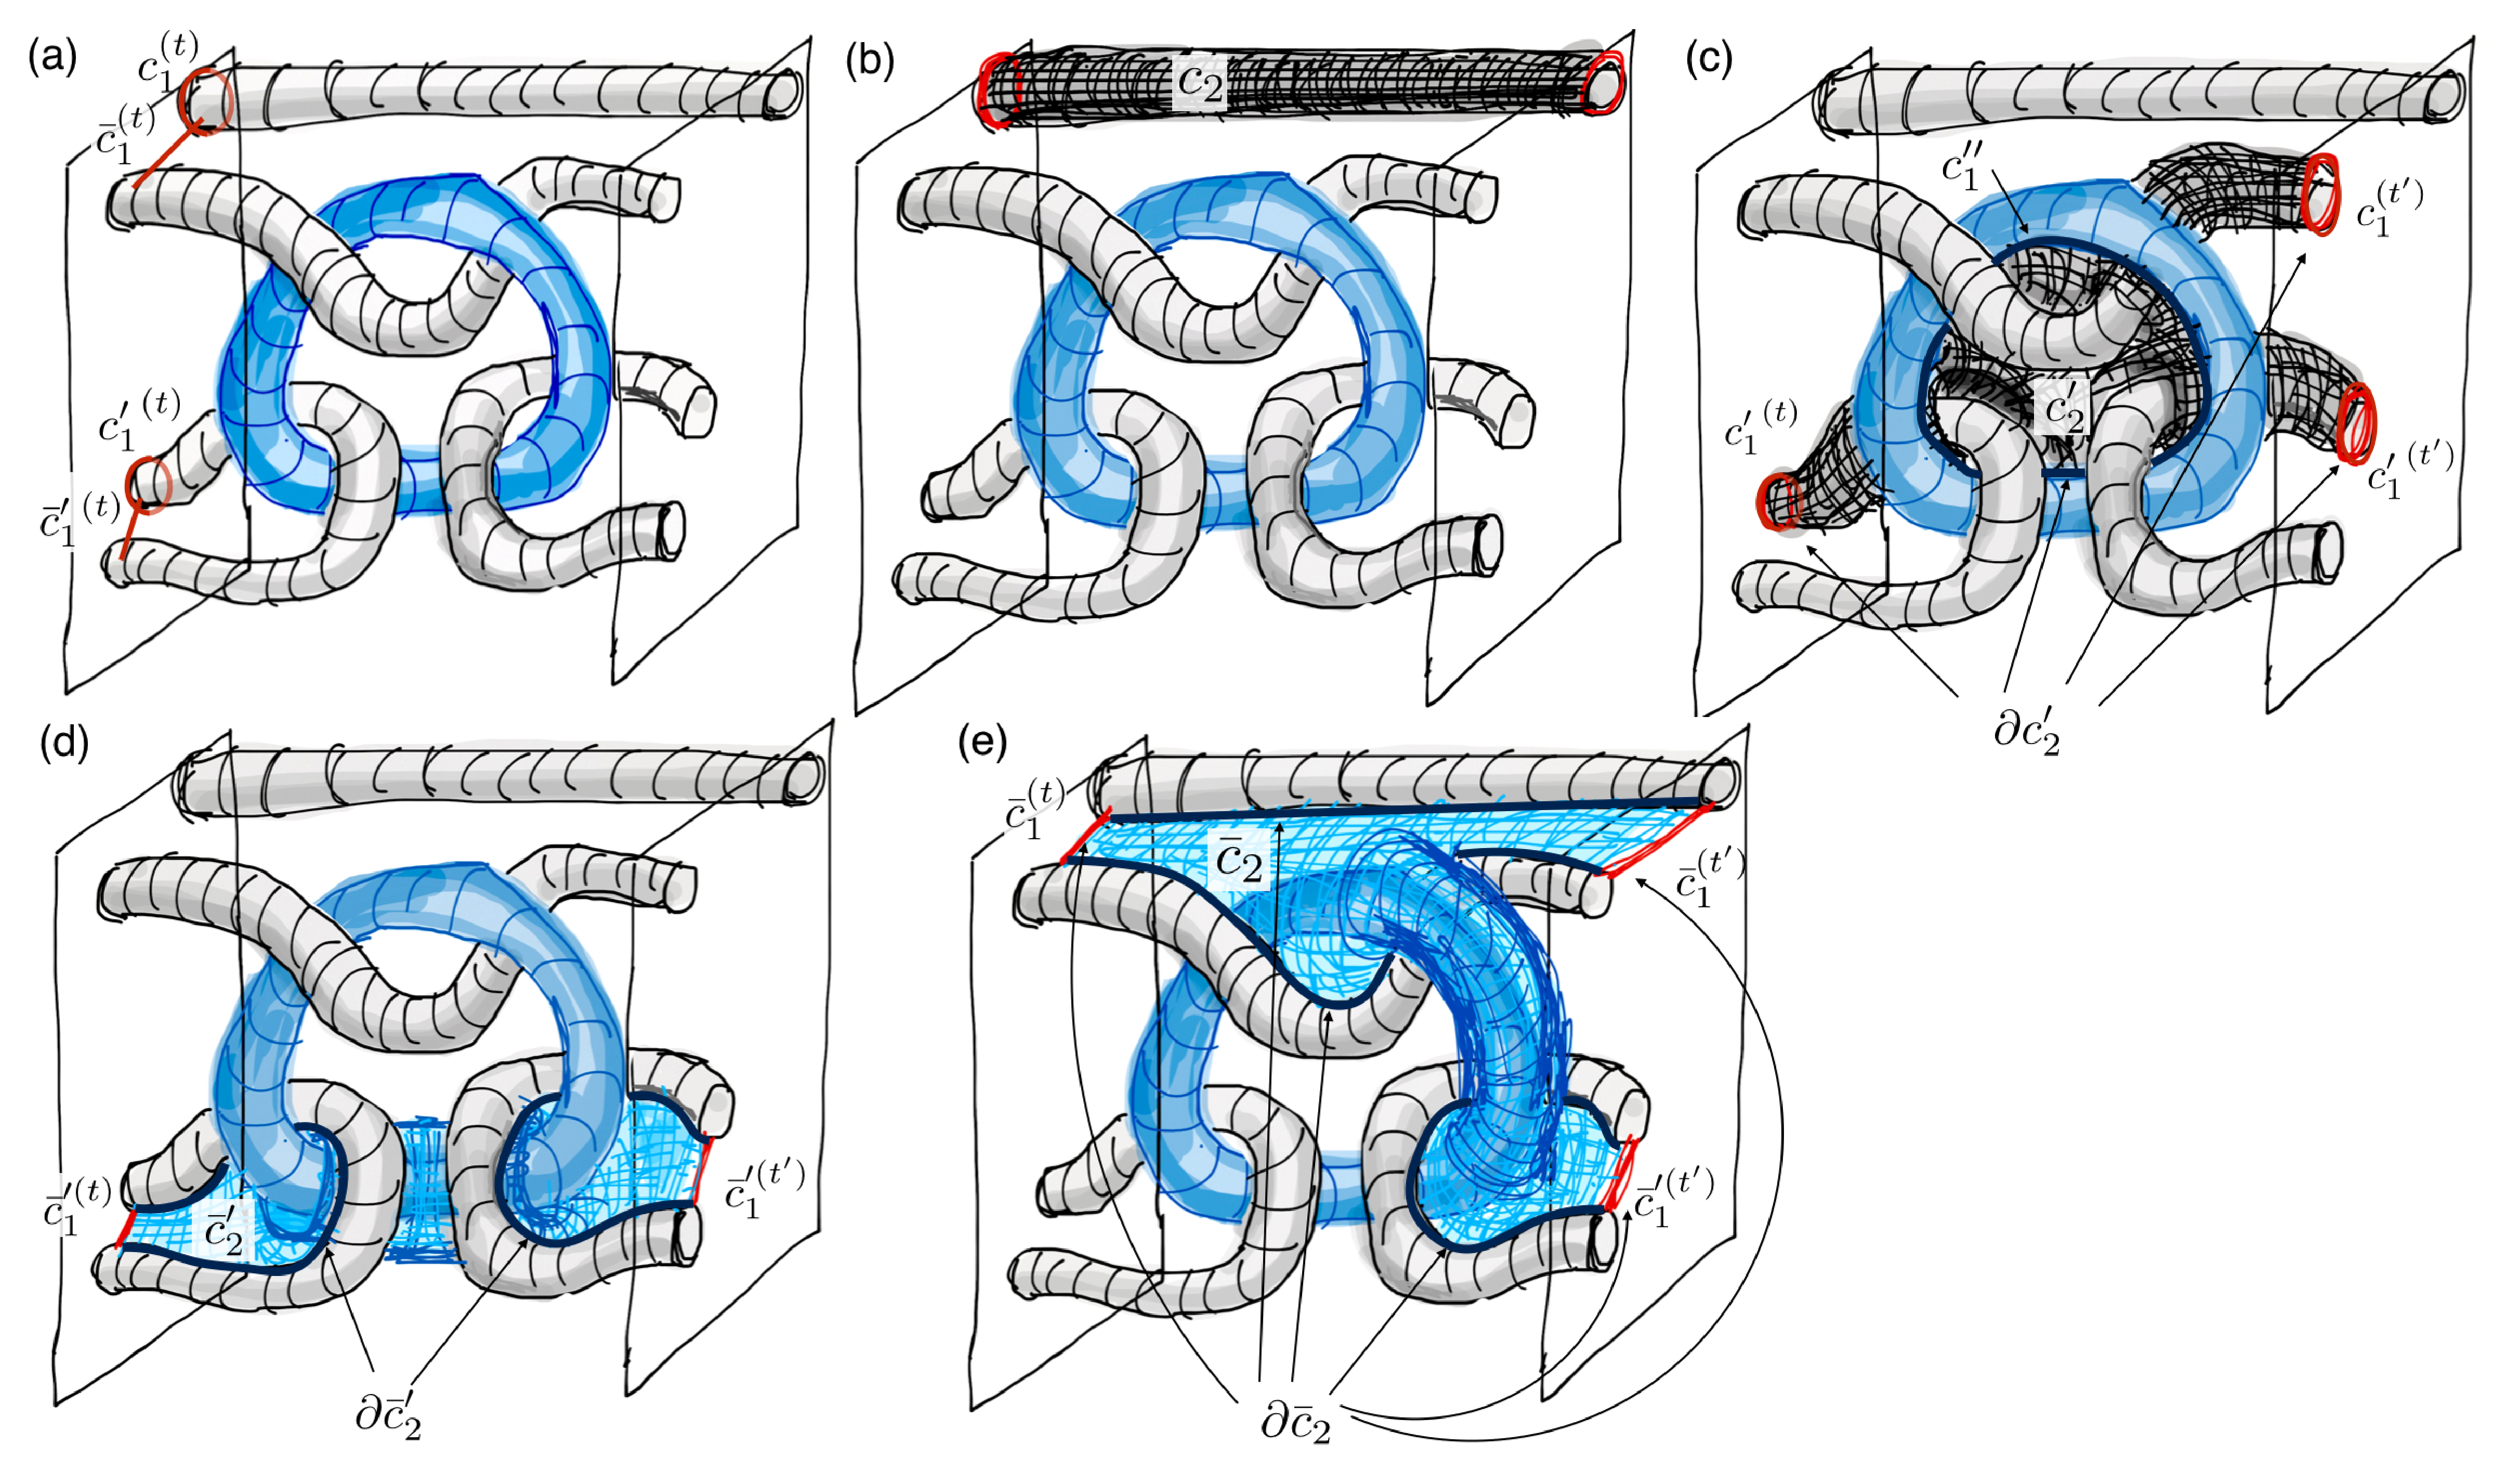
\includegraphics[width=140mm]{figAp09.eps}
\caption{(a) A diagram for defect braiding for a logical CNOT gate.
(b-e) Time evolutions of the logical operators and the corresponding correlation surfaces.}
\label{figAp09}
\end{figure*}
%%%%
\subsection*{CNOT gate by braiding}
Let us consider primal defects braiding around a dual defect as shown in Fig.~\ref{figAp09} (a).
Similarly to the previous case, we calculate the time evolution of logical operators by the measurements.
The state at time step $t$ is described by $\{ L_Z^{(t)}, L_X^{(t)}\}$ and $\{ {L'_Z}^{(t)}, {L'_X}^{(t)}\}$ corresponding to $\{ c_1^{(t)}, \bar c_1^{(t)}\}$ and 
$\{ {c'_1}^{(t)}, {{\bar c}'_1}{}^{(t)} \}$, respectively.
We first consider a correlation surface $c_2$ with respect to $c_1^{(t)}$, as depicted in Fig.~\ref{figAp09} (b). 
Similarly to the identity gate, $L_Z^{(t)}$ is transformed into ${L'}_Z^{(t)}$.
An interesting thing happens when we consider the correlation surface $c'_2$ with respect to ${c'_1}^{(t)}$, as shown in Fig.~\ref{figAp09} (c).
The stabilizer operator on $c'_2$ is given by 
\begin{eqnarray}
K(c'_2) &=& Z(\partial c'_2) X( c'_2)
\nonumber \\
&=& Z({c'_1}^{(t)}) Z({c_1}^{(t')}) Z({c'_1}^{(t')}) Z(c''_1) X(c'_2) ,
\end{eqnarray}
where $c''_1$ is a cycle in the dual defect of a loop as shown in Fig.~\ref{figAp09} (c).
Then after the measurements, we obtain an equivalence relation,
\begin{eqnarray}
L_Z^{(t)} \sim {L}_Z^{(t')} {L'}_Z^{(t')}.
\end{eqnarray}
Note that inside the dual defect region, the dual face (primal edge) qubits are measured in the $Z$-basis, and hence we can obtain the eigenvalue of $Z(c''_1)$.
After a similar argument using a defect surface $\bar c_2$ and $\bar c'_2$ with respect to the dual 1-chain $\bar c_1$ and $\bar c'_1$, shown in Fig.~\ref{figAp09} (d) and (e), respectively, we obtain 
\begin{eqnarray}
L_X^{(t)} &\sim& {L}_X^{(t)},
\\
L_X^{(t')} &\sim& {L}_X^{(t')} {L'}_X^{(t')}.
\end{eqnarray}
These relations between the logical operators at time steps $t$ and $t'$ are equivalent to those for the CNOT gate.
Thus, the defect braiding in Fig.~\ref{figAp09} results in a logical CNOT gate.
Now we realize that the correlation surface 
introduced in Chapter~\ref{Chap:TQC} 
as a trajectory of the logical operator 
corresponds to the correlation surface defined by the 
stabilizer operator of the cluster state.

\subsection*{A singular qubit injection for magic state distillation}
So far, we have shown that the Clifford circuits, Pauli-basis preparation, measurements, and CNOT gate, can all be implemented in a topological way.
Unfortunately, these operations are not enough to generate universal quantum computation.
To implement universal quantum computation, we inject $Y$- and $(X+Y)/\sqrt{2}$-basis states by measuring singular qubits in the $Y$- and $(X+Y)/\sqrt{2}$-bases, respectively, as shown in Fig.~\ref{figAp10}.
Let us see how this measurement works.
Similarly to the previous case, we have two correlation surfaces $c_2$ and $\bar c_2$:
\begin{eqnarray}
K(c_2) &=& Z(\partial c_2) X(c_2) = Z(\partial c_2) X(c_2 \backslash s) X_s,
\\
K(\bar c_2) &=& Z(\partial \bar c_2) X(\bar c_2 ) =Z_s Z(\partial \bar c_2\backslash s) X(\bar c_2 ),
\end{eqnarray}
where $A_s$ is a Pauli operator on the singular qubit and $[\cdot]\backslash s$ indicates a chain with a removal of an element corresponding to the singular qubit.
Suppose the singular qubit is measured in the $Y$-basis.
After the measurements, the state at time step $t$ is stabilized by
\begin{eqnarray}
K(c_2) K(\bar c_2) \simeq L_X^{(t)}L_Z^{(t)} \equiv L_Y^{(t)}.
\end{eqnarray}
Thus, a logical $Y$-basis state is prepared.
When the singular qubit is measured in the $(X+Y)/\sqrt{2}$-basis, the state at time step $t$ is stabilized by
\begin{eqnarray}
[ K(\bar c_2) + K(c_2) K(\bar c_2)]/\sqrt{2} \simeq (L_X^{(t)}+ L_Y^{(t)})/\sqrt{2},
\end{eqnarray}
which means that a logical $(X+Y)/\sqrt{2}$-basis state is prepared.
%%%%
\begin{figure}[t]
\centering
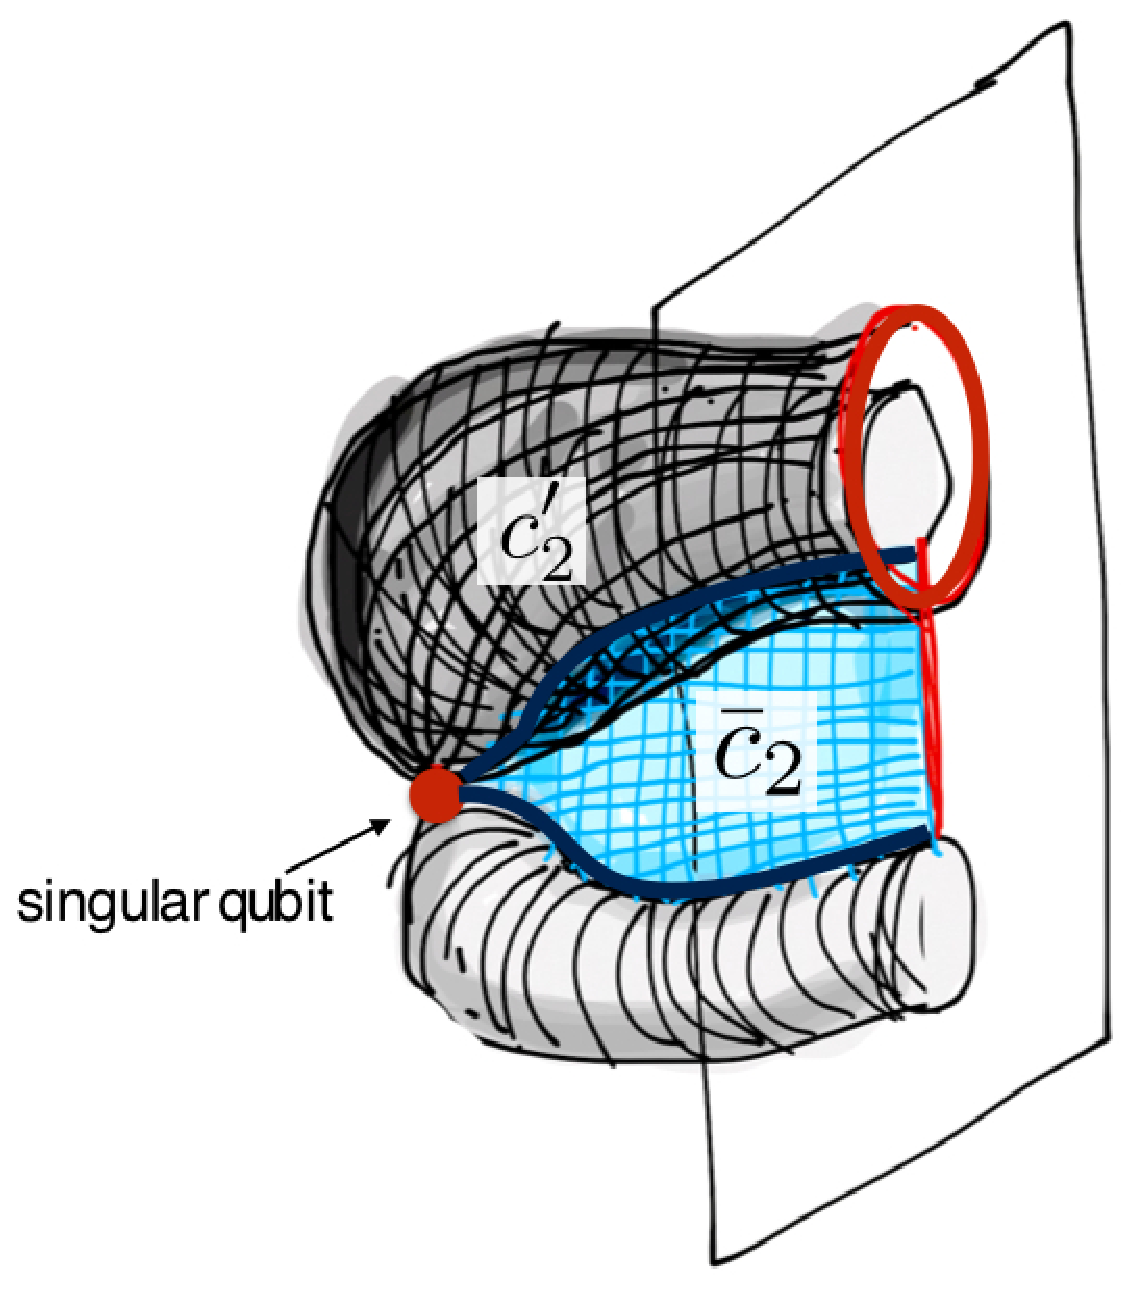
\includegraphics[width=70mm]{figAp10.eps}
\caption{A state injection on the singular qubit.}
\label{figAp10}
\end{figure}
%%%%

These states are utilized to implement $S$, $T$, $HSH$, and $HTH$ gates using gate teleportation with the CNOT gate.
These gates form a universal set of gates.

\section{Topological quantum error correction in 3D}
Next, we will see how topological quantum error correction is
done in 3D.
Indeed, in the 3D case, 
the argument for the noisy syndrome measurements 
made in Chapter~\ref{Chap:TQC}
becomes more simple as follows.
All measurements in the vacuum region are done in the $X$-basis.
We consider a stabilizer operator on a unit primal cube $q$,
\begin{eqnarray}
K(\partial q_n) = \prod _{f_m \in \partial q_n } X_{f_m},
\end{eqnarray}
where there is no $Z$ operator due to $\partial \circ \partial q_n =0$.
This implies that, if there is no error, the parity of each six $X$-basis measurement outcomes on the primal cube is always even.
The errors are described by using a dual 1-chain $E=Z(\bar c_1)$.
At a unit cube $q_n$ belonging to $\partial \bar c_1$, 
we have 
$|q_n \cap \partial \bar c_1 |={\rm odd}$.
(Recall that the primal $3$-chain and the dual $0$-chain are identified.)
From a set of odd parity cubes $\partial \bar c_1$, we estimate the actual location of errors $E' = Z(\bar c'_1)$ such that $\partial \bar c_1 = \partial \bar c'_1$.
If the total of the actual and estimated error chains $\bar c_1 + \bar c'_1$ results in a trivial cycle, meaning that there is no defect inside the cycle, it can be contracted and removed by a continuous deformation.
If the total of the actual and estimated error chains $\bar c_1 + \bar c'_1$ results in a nontrivial cycle, meaning a cycle winding around a defect, $EE'=Z(\bar c_1 + \bar c'_1)$ may result in a logical operator. 
In such a case, the topological error correction has failed.
This property is completely the same as the topological quantum error correction
under faulty syndrome measurements 
argued in Sec.~\ref{Sec:TopoFaultTolerance}.
If the error probability is smaller than a constant value (the threshold), the failure probability of the topological quantum error correction decreases exponentially in the characteristic size and distance of the defects.

Inside the defect region, the face qubits are measured in the $Z$-basis.
Especially, the $Z$-basis measurement outcomes near the defect boundary are employed to evaluate the correlation surface.
Note that these $Z$-basis measurements and the removal of the corresponding bonds of the cluster state can instead be done by generating a cluster without connecting the corresponding bonds in advance.
In such a case, the errors on the $Z$-basis measurements do not appear.
We can obtain an additional parity $K_{f_m}$ and $K_{\bar f_{m'}}$ at the primal and dual faces on the boundary of the defects, respectively.
If the errors on the face qubits ${f_m}$ and $\bar f_{m'}$ are suppressed, the errors on the boundary are reduced into errors on a toric code on a 2D surface, $\partial D$ or 
$\partial \bar D$.
Again, if the error probability is sufficiently smaller than a constant threshold value, we can correct it faithfully.

The $X$- and $Z$-basis state preparations and measurements, and the CNOT gate obtained by braiding, are topologically protected because we can execute these topological operations by keeping the defect size and distance larger than an arbitrarily large constant length.
Unfortunately, through the state injection, we shrink the defect size into an elementary unit cell, where the defect size and distance become very small.
Thus, the topological protection is broken down around the singular qubit (see Fig.~\ref{figAp10} (a)). 
There will also be lower weight errors, which effectively increase the logical error probability on the injected logical states.
However, noisy injected states can be purified by using the topologically protected Clifford gates, the so-called magic state distillation.
The $Y$- and $(X+Y)/\sqrt{2}$-basis states are distilled by using the 7-qubit Steane and 15-qubit Reed-Muller codes, respectively
as explained.
The distilled states are utilized to implement non-Clifford gates via gate teleportation, as seen before.
In this way, universal quantum computation is executed with arbitrary accuracy.



\section{Applications for MBQC on thermal states}
Topologically protected MBQC in 3D is useful to study the quantum computational capacity of quantum many-body states at finite temperature.
Consider the stabilizer Hamiltonian of the 3D cluster state for topological MBQC \cite{MBQC_PRA,RaussendorfBravyi,BarrettThermal}:
\begin{eqnarray}
H_{\rm fc} = -J \left[ \sum _{f} K(f) + \sum_{\bar f}  K(\bar f) \right].
\end{eqnarray}
The thermal state at temperature $T=1/(\beta J)$ is given by
\begin{eqnarray}
\rho _{\rm fc} &=& e^{ - \beta H_{\rm fc} } / {\rm Tr}[e^{ - \beta H _{\rm fc} }].
\end{eqnarray}
Using a unitary operator $U_{CZ}= \prod _{(f_m,\bar f_l ) } \Lambda_{f_m,\bar f_l}(Z)$, consisting of $CZ$ gates on all nearest-neighbor two qubits, the thermal state can be mapped into the thermal state of an interaction-free spin model:
\begin{eqnarray}
U_{CZ} \rho _{\rm fc} U_{CZ}^{\dag}
=
e^{ - \beta H_{\rm f}   } / {\rm Tr}[e^{ - \beta H _{\rm f} }] ,
\end{eqnarray}
where 
\begin{eqnarray}
H_{\rm f} \equiv  -J \sum _{i} X_i = U_{CZ} H_{\rm fc} U_{CZ}^{\dagger}.
\end{eqnarray}
Because $H_{\rm f}$ is an interaction-free Hamiltonian, the stabilizer Hamiltonian, which we will call the {\it free cluster Hamiltonian}, does not undergo any thermodynamic phase transition.

The thermal state of the free cluster Hamiltonian is given as a product state of the single-spin density matrix:
\begin{eqnarray}
\rho _{\rm f} &=& e^{- \beta H_{\rm f}}/{\rm Tr}[e^{- \beta H_{\rm f}}] = \prod _{i} e^{\beta J X_i}/{\rm Tr}[e^{\beta J X_i}]
\\
&=& \prod _{i} \mathcal{E}_i(p_{\beta J}) (|+\rangle \langle +|)^{\otimes n},
\end{eqnarray}
where 
\begin{eqnarray}
\mathcal{E}_i(p) = (1-p) \rho + p Z_i \rho Z_i,
\end{eqnarray}
and $p_{\beta J} = e^{- 2 \beta J }/(1+e^{- 2 \beta J })$.
Because $\mathcal{E}_i$ and $U_{CZ}$ commute, the thermal state of $H_{\rm fc}$ is rewritten as
\begin{eqnarray}
\rho _{\rm fc} = U_{CZ} \rho _{\rm f} U_{CZ} ^{\dag} =\left[ \prod _{i} \mathcal{E}_i (p_{\beta J}) \right] U_{CZ} (|+\rangle \langle +|)^{\otimes n} U_{CZ}^{\dag}
=\left[ \prod _{i} \mathcal{E}_i (p_{\beta J}) \right]  |\Psi _{3D} \rangle \langle \Psi _{3D} |,
  \nonumber
\\
\end{eqnarray}
where $|\Psi _{3D}\rangle$ is the ground state of $H_{\rm fc}$, i.e., the 3D cluster state.
This means that the thermal state is given as an ideal 3D cluster state, followed by an independent dephasing for each qubit with probability 
$p_{\beta J}=e^{- 2 \beta J }/(1+e^{- 2 \beta J })$.
From the argument made in the previous section, if $p \leq 2.9-3.3\%$ and hence $T = 1/(\beta J) \leq 0.57-0.59$, we can then perform universal quantum computation reliably on the thermal state at a finite temperature, where the errors originating from the thermal excitations are corrected by the topological quantum error correction.
On the other hand, in the high temperature limit $T=1/(\beta J) \rightarrow \infty$, the thermal state is given by a completely mixed state, and hence MBQC on it can be simulated classically.

A projected-entangled-pair state (PEPS)\index{projected-entangled-pair state, PEPS} picture~\cite{PEPS,RaussendorfBravyi,BarrettThermal} allows us to obtain a lower bound for the possibility of a classical simulation.
In the PEPS picture, the 3D cluster state is described as follows.
A maximally entangled pair $|\psi _{\rm MES}\rangle \equiv (|0\rangle |+\rangle + |1\rangle |-\rangle)/\sqrt{2}$ is shared on each bond.
On each site consisting of halves of the entangled pair, a projection 
\begin{eqnarray}
|0\rangle \langle 00..0| + |1\rangle \langle 11..1|
\end{eqnarray}
is performed with an appropriate normalization.
The resultant state is the 3D cluster state.
Because the projection and the $Z$ error $\mathcal{E}_i$ commute, the effect of the thermal excitations on the shared entangled state can be determined beforehand:
\begin{eqnarray}
\rho_{\rm bond} =\mathcal{E}_a(p)\mathcal{E}_b(p) |\psi _{\rm MES}\rangle \langle \psi _{\rm MES}|
\end{eqnarray}
If $p \geq (2-\sqrt{2})/2$, the decohered entangled pair $\rho _{\rm bond}$ becomes a separable state.
If two bonds per site are made separable, the 3D cluster state becomes a separable state.
A sampling on such a resource state can be simulated efficiently classically~\cite{BarrettThermal,FujiiTamate}.
In this case, the $Z$ error probability per site has to be $p_{\beta J} \geq \sqrt{2}-1$, i.e., $T= 1/(\beta )=5.77J$.
The true critical temperature $T_c$ between the classically simulatable and universal quantum computational phases is located in the range $0.59J<T_c < 5.77J$.
Note that this model exhibits a transition of the computational capability, while there is no thermodynamic phase transition in the physical system~\cite{RaussendorfBravyi,BarrettThermal}.
%%%%
\begin{figure}[t]
\centering
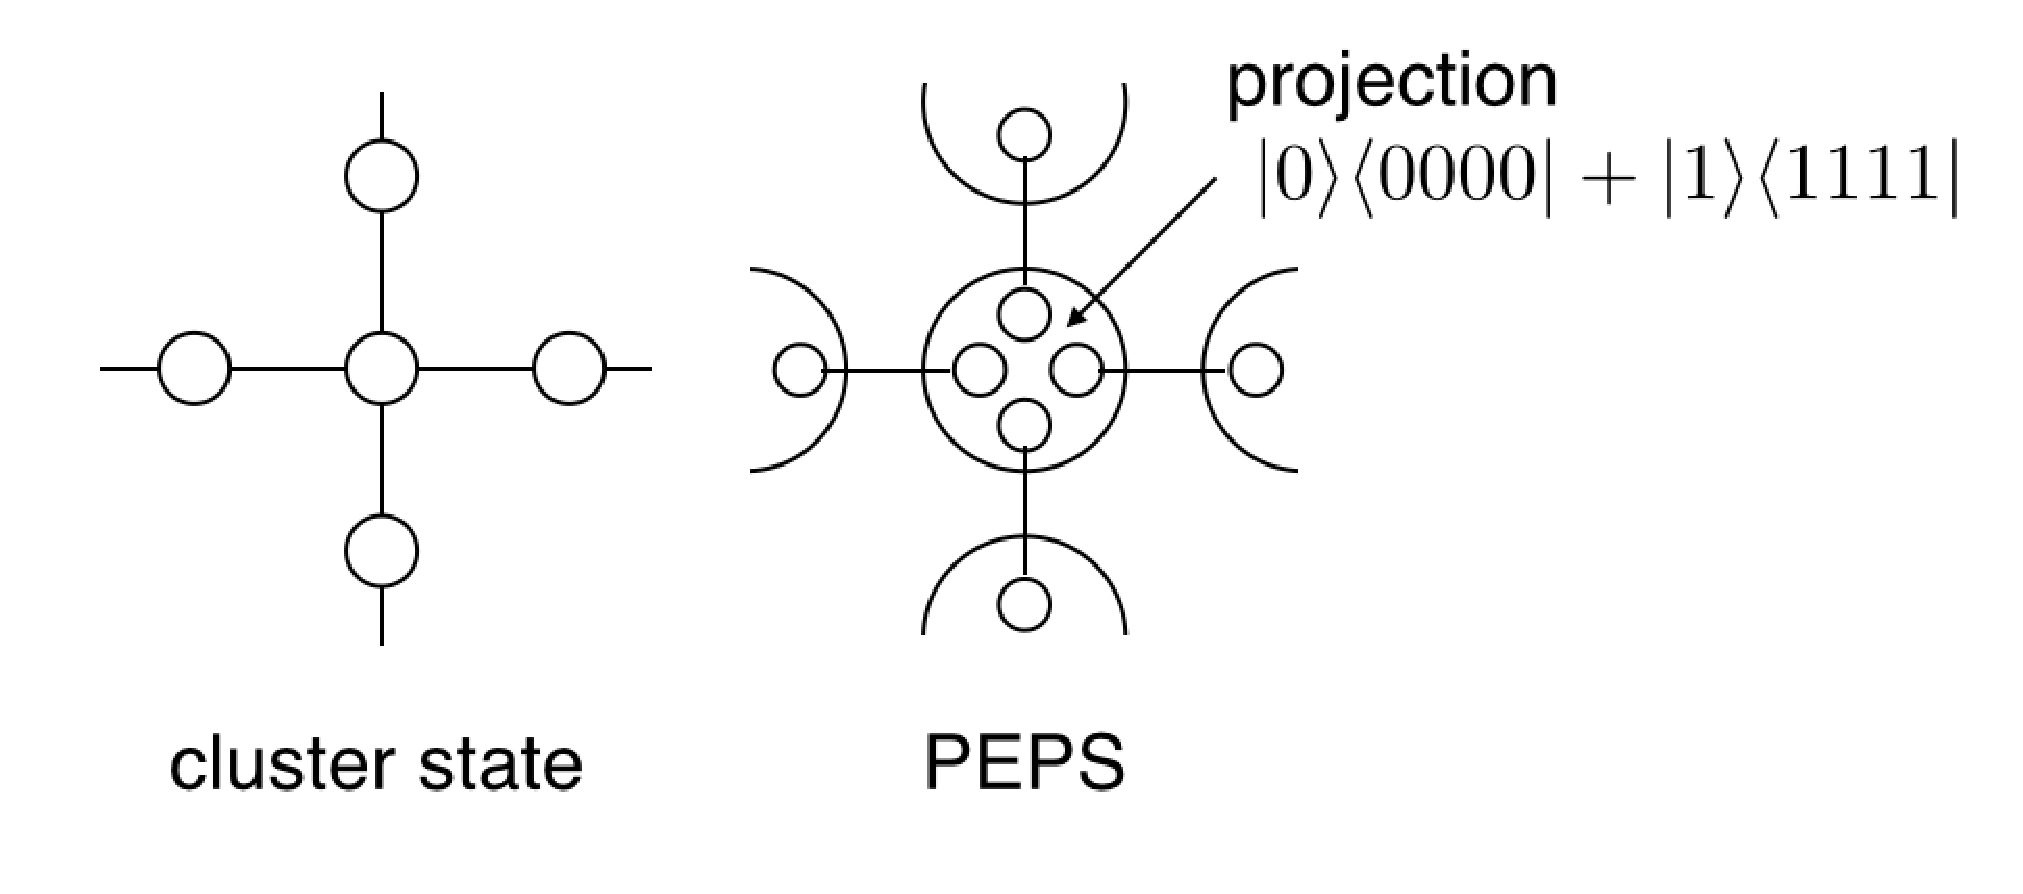
\includegraphics[width=100mm]{fig92.eps}
\caption{A PEPS picture of the cluster state.}
\label{fig92}
\end{figure}
%%%%

In classical information processing, a thermodynamic phase transition, or, more precisely, an ordered phase below a critical temperature is utilized for robust information storage in magnetic storage devises.
While there is no such long range order in the previous model, it is natural to ask whether or not a long range ordered phase is useful to enhance the measurement-based quantum computation on many-body thermal states for quantum information processing.
To address this issue, Fujii {\it et al.} proposed an interacting cluster Hamiltonian \cite{FujiiNakata},
\begin{eqnarray*}
H_{\rm ic} = -J \sum _{\langle f,\bar f \rangle } K(f)K(\bar f).
\end{eqnarray*}
Because interactions are introduced between the cluster stabilizers, this model is mapped by $U_{CZ}$ into an Ising model on a 3D lattice:
\begin{eqnarray*}
H_{\rm Ising} = U_{CZ}H_{\rm ic} U_{CZ}^{\dag} 
= -J \sum _{\langle f,\bar f \rangle } X_f X_{\bar f}.
\end{eqnarray*}
Thus, it undergoes a thermodynamic phase transition at a finite temperature.
The degenerate ground states
\begin{eqnarray}
U_{CZ}|+\rangle^{\otimes n} \textrm{ and } U_{CZ}|-\rangle^{\otimes n}
\end{eqnarray} 
are also the 3D cluster states, up to the simultaneous spin flipping due to the global symmetry.
Because the eigenvalues of the cluster stabilizer have a long range order (they are likely to be aligned in the same direction) in a ferromagnetic ordered phase, the topologically protected MBQC on the symmetry-breaking thermal state has a special robustness against the thermal excitations.
In Ref.~\cite{FujiiNakata}, topological quantum error correction of this model is mapped to a correlated random plaquette $\mathbf{Z}_2$-gauge model in 3D, where the disorder in the signs of the plaquettes has an Ising-type correlation.
By using this property and the gauge transformation on the Nishimori line \cite{NishimoriBook}, Fujii {\it et al.} showed that the critical temperature of this model, and hence the threshold temperature for topological protection, is equal to the critical temperature of the 3D Ising model, which is the unitary equivalent model of the interacting cluster Hamiltonian.
This means that the critical temperatures for the topological protection and the thermodynamic phase transition of the underlying physical system coincides exactly.
Due to this fact, we can improve the threshold temperature for topological protection by one order of magnitude.

While the above Hamiltonian employs multi-body interactions, the 3D cluster state can be generated from the thermal states of a nearest-neighbor two-body Hamiltonian for spin-3/2 and composite spin-1/2 particles via local filtering operations \cite{LiKwek,FujiiMoriTher}.
Let us consider a system consisting of a spin-3/2 particle located at site $\mathbf{r}$ and a composite particle of two spin-1/2 particles located at the nearest-neighbor site $\mathbf{r}+\mathbf{i}$, with $\mathbf{i}=\mathbf{1},\mathbf{2},\mathbf{3}$, as shown in Fig~\ref{fig93} (a).
The Hamiltonian is given by
\begin{eqnarray*}
 H&=& \Delta  \sum _{\mathbf{r}} \vec{S} _{\mathbf{r}} \cdot (\vec{I}_{ \mathbf{r} + \mathbf{1}}+\vec{I}_{\mathbf{r} +\mathbf{2}}+ \vec{I}_{\mathbf{r} +\mathbf{3}} )
\end{eqnarray*}
where $\vec{S}_{\mathbf{r}} \equiv (S_{\mathbf{r}}^x,S_{\mathbf{r}}^y,S_{\mathbf{r}}^z)$ is the spin-3/2 operator of the center particle at the position $\mathbf{r}$ and $\vec{I}_{\mathbf{r} + \mathbf{a}} = \vec A _{\mathbf{r} + \mathbf{a}} $ or $\vec B_{\mathbf{r}+ \mathbf{a}}$ depending on the interaction types (line or dash). 
Here, $\vec A _{\mathbf{r} + \mathbf{a}}\equiv (A_{\mathbf{r} +\mathbf{a}}^x,A_{\mathbf{r} +\mathbf{a}}^y,A_{\mathbf{r}+\mathbf{a}}^z)$ and 
$\vec B_{\mathbf{r}+ \mathbf{a}}\equiv (B_{\mathbf{r} +\mathbf{a}}^x,B_{\mathbf{r} +\mathbf{a}}^y,B_{\mathbf{r}+\mathbf{a}}^z)$ are two independent spin-1/2 operators on the composite particle at the position $\mathbf{r} + \mathbf{a}$ ($\mathbf{a} = \mathbf{1} , \mathbf{2}, \mathbf{3}$).
The above Hamiltonian $H$ can be reformulated as
\begin{eqnarray*}
H
&=&  \sum _{\mathbf{r}} H_{\mathbf{r}} =\Delta /2 \sum _{\mathbf{r}}
( \vec{T}^2  _{\mathbf{r}} - \vec{S}^2 _{\mathbf{r}}  -  \vec {I}_{\mathbf{r}} ^2)
 \end{eqnarray*}
where $\vec{I}_{\mathbf{r}} \equiv  \vec{I} _{\mathbf{r} + \mathbf{1}}+\vec{I} _{\mathbf{r} + \mathbf{2}}+\vec{I} _{\mathbf{r} + \mathbf{3}}$ and 
$\vec T _{\mathbf{r}} \equiv \vec S_{\mathbf{r}} + \vec I _{\mathbf{r}}$.
The ground state $|G \rangle = \bigotimes _{\mathbf{r}} |g_{\mathbf{r}} \rangle$ is given by $T_{\mathbf{r}} =0$, $S_{\mathbf{r}} =3/2$, and $I_{\mathbf{r}} =3/2$, where $L_{\mathbf{r}}(L_{\mathbf{r}}+1)$ ($L=T,S,I$) is the eigenvalue of the operator $\vec L_{\mathbf{r}}^2$.
%(i.e. $L_{\mathbf{r}}$  indicates the sipn angular momentum quantum number).
Each center particle in the ground state $|G\rangle$ is filtered by using the POVM measurement: 
\begin{eqnarray}
\{ F^{\alpha}= ({S_{\mathbf{r}} ^\alpha} ^2 - 1/4)/\sqrt{6} \} \;\;\; (\alpha =x,y,z).
\end{eqnarray}
If the measurement outcome is $\alpha =z$, we obtain a four-qubit GHZ (Greenberger-Horne-Zeilinger) state
~\cite{GHZ} as the post-POVM measurement state: 
\begin{eqnarray*}
|{\rm GHZ} ^4_{\mathbf{r}} \rangle  \equiv \frac{1}{\sqrt{2}} (|\tilde 0 +++\rangle + |\tilde 1 ---\rangle) ,
\end{eqnarray*}
where $|\tilde 1 \rangle  $ and $|\tilde 0 \rangle $ are eigenstates of $S^z$ with eigenvalues $+3/2$ and $-3/2$, respectively, and $|\pm\rangle$ are the eigenstates of $A^{z}$ or $B^{z}$ with eigenvalues $\pm 1$, respectively.
Even if we obtain other outcomes, we can transform the post-POVM measurement state to $|{\rm GHZ} ^4_{\mathbf{r}}\rangle$ by local operations.
The four-qubit GHZ state is subsequently used to construct the 2D honeycomb cluster state, which is a universal resource for MBQC, by measuring the operators $A^z \otimes B^x$ and $A^x \otimes B^z$ on the bond particle
as shown in Fig.~\ref{fig93} (a).

In the case of finite temperature, we have the thermal state $\bigotimes _{\mathbf{r}} \rho _{\mathbf{r}}$ with 
$\rho _{\mathbf{r}} \equiv e^{ - \beta  H_{\mathbf{r}} } /\mathcal{Z} $ instead of the ground state, where $\mathcal{Z}$ indicates the partition function and $\beta = T ^{-1}$ for a temperature $T$.  
Then, the GHZ state becomes a noisy, say thermal, GHZ state, 
$\sigma _{\mathbf{r}} \equiv F^{\alpha } \rho _{\mathbf{r}} {  F^{\alpha}} ^{\dag}/{\rm Tr}[ F^{\alpha } \rho _{\mathbf{r}}{  F^{\alpha}} ^{\dag}]$.
In the low temperature case, the thermal GHZ state 
is calculated, in the leading order, to be
 $\mathcal{E}_4 (|{\rm GHZ} ^4_{\mathbf{r}} \rangle  \langle {\rm GHZ} ^4_{\mathbf{r}}| )$ with 
\begin{eqnarray}
\mathcal{E}_4 &=& (1- q_1 - 3q_2 - 3q_3 ) [I] + q_1 [Z_{\mathbf{r}}  ]
\nonumber \\&&
+q_2 \sum _{\mathbf{a}=\mathbf{1},\mathbf{2},\mathbf{3}} [Z_{\mathbf{r} + \mathbf{a}}] 
+q_3 \sum _{\mathbf{a}=\mathbf{1},\mathbf{2},\mathbf{3}} [Z_{\mathbf{r} }Z_{\mathbf{r} + \mathbf{a}}] ,
\label{error}
\end{eqnarray}
where $q_1$, $q_2$, and $q_3$ are the error probabilities as functions of the temperature $T$, the Pauli $Z$ operator $Z_{\mathbf{b}}$ on the qubit at the position $\mathbf{b}$, and $[C]\rho \equiv C \rho C^{\dag}$, respectively.
The probability of other errors such as $Z_{\mathbf{r}} Z_{\mathbf{r} +\mathbf{a}} Z_{\mathbf{r} +\mathbf{a} '}$ is several orders of magnitude smaller than $q_{1,2,3}$.

To obtain the 3D cluster state for topological MBQC, as done in Ref.~\cite{LiKwek}, the five-qubit GHZ state $|{\rm GHZ}^5_{\mathbf{r}}\rangle$ is generated in a similar way by using spin-2 particles and composite particles of spin-1/2, as shown in Fig.~\ref{fig93} (b).
Instead of the spin-2 particles, spin-3/2 particles were employed in Ref.~\cite{FujiiMoriTher} to obtain the 3D cluster state shown in Fig.~\ref{fig93} (c).
After the filtering operation and local operations, the two four-qubit GHZ states are connected to obtain the five-qubit GHZ state for building the 3D cluster state.
%%%%
\begin{figure}[t]
\centering
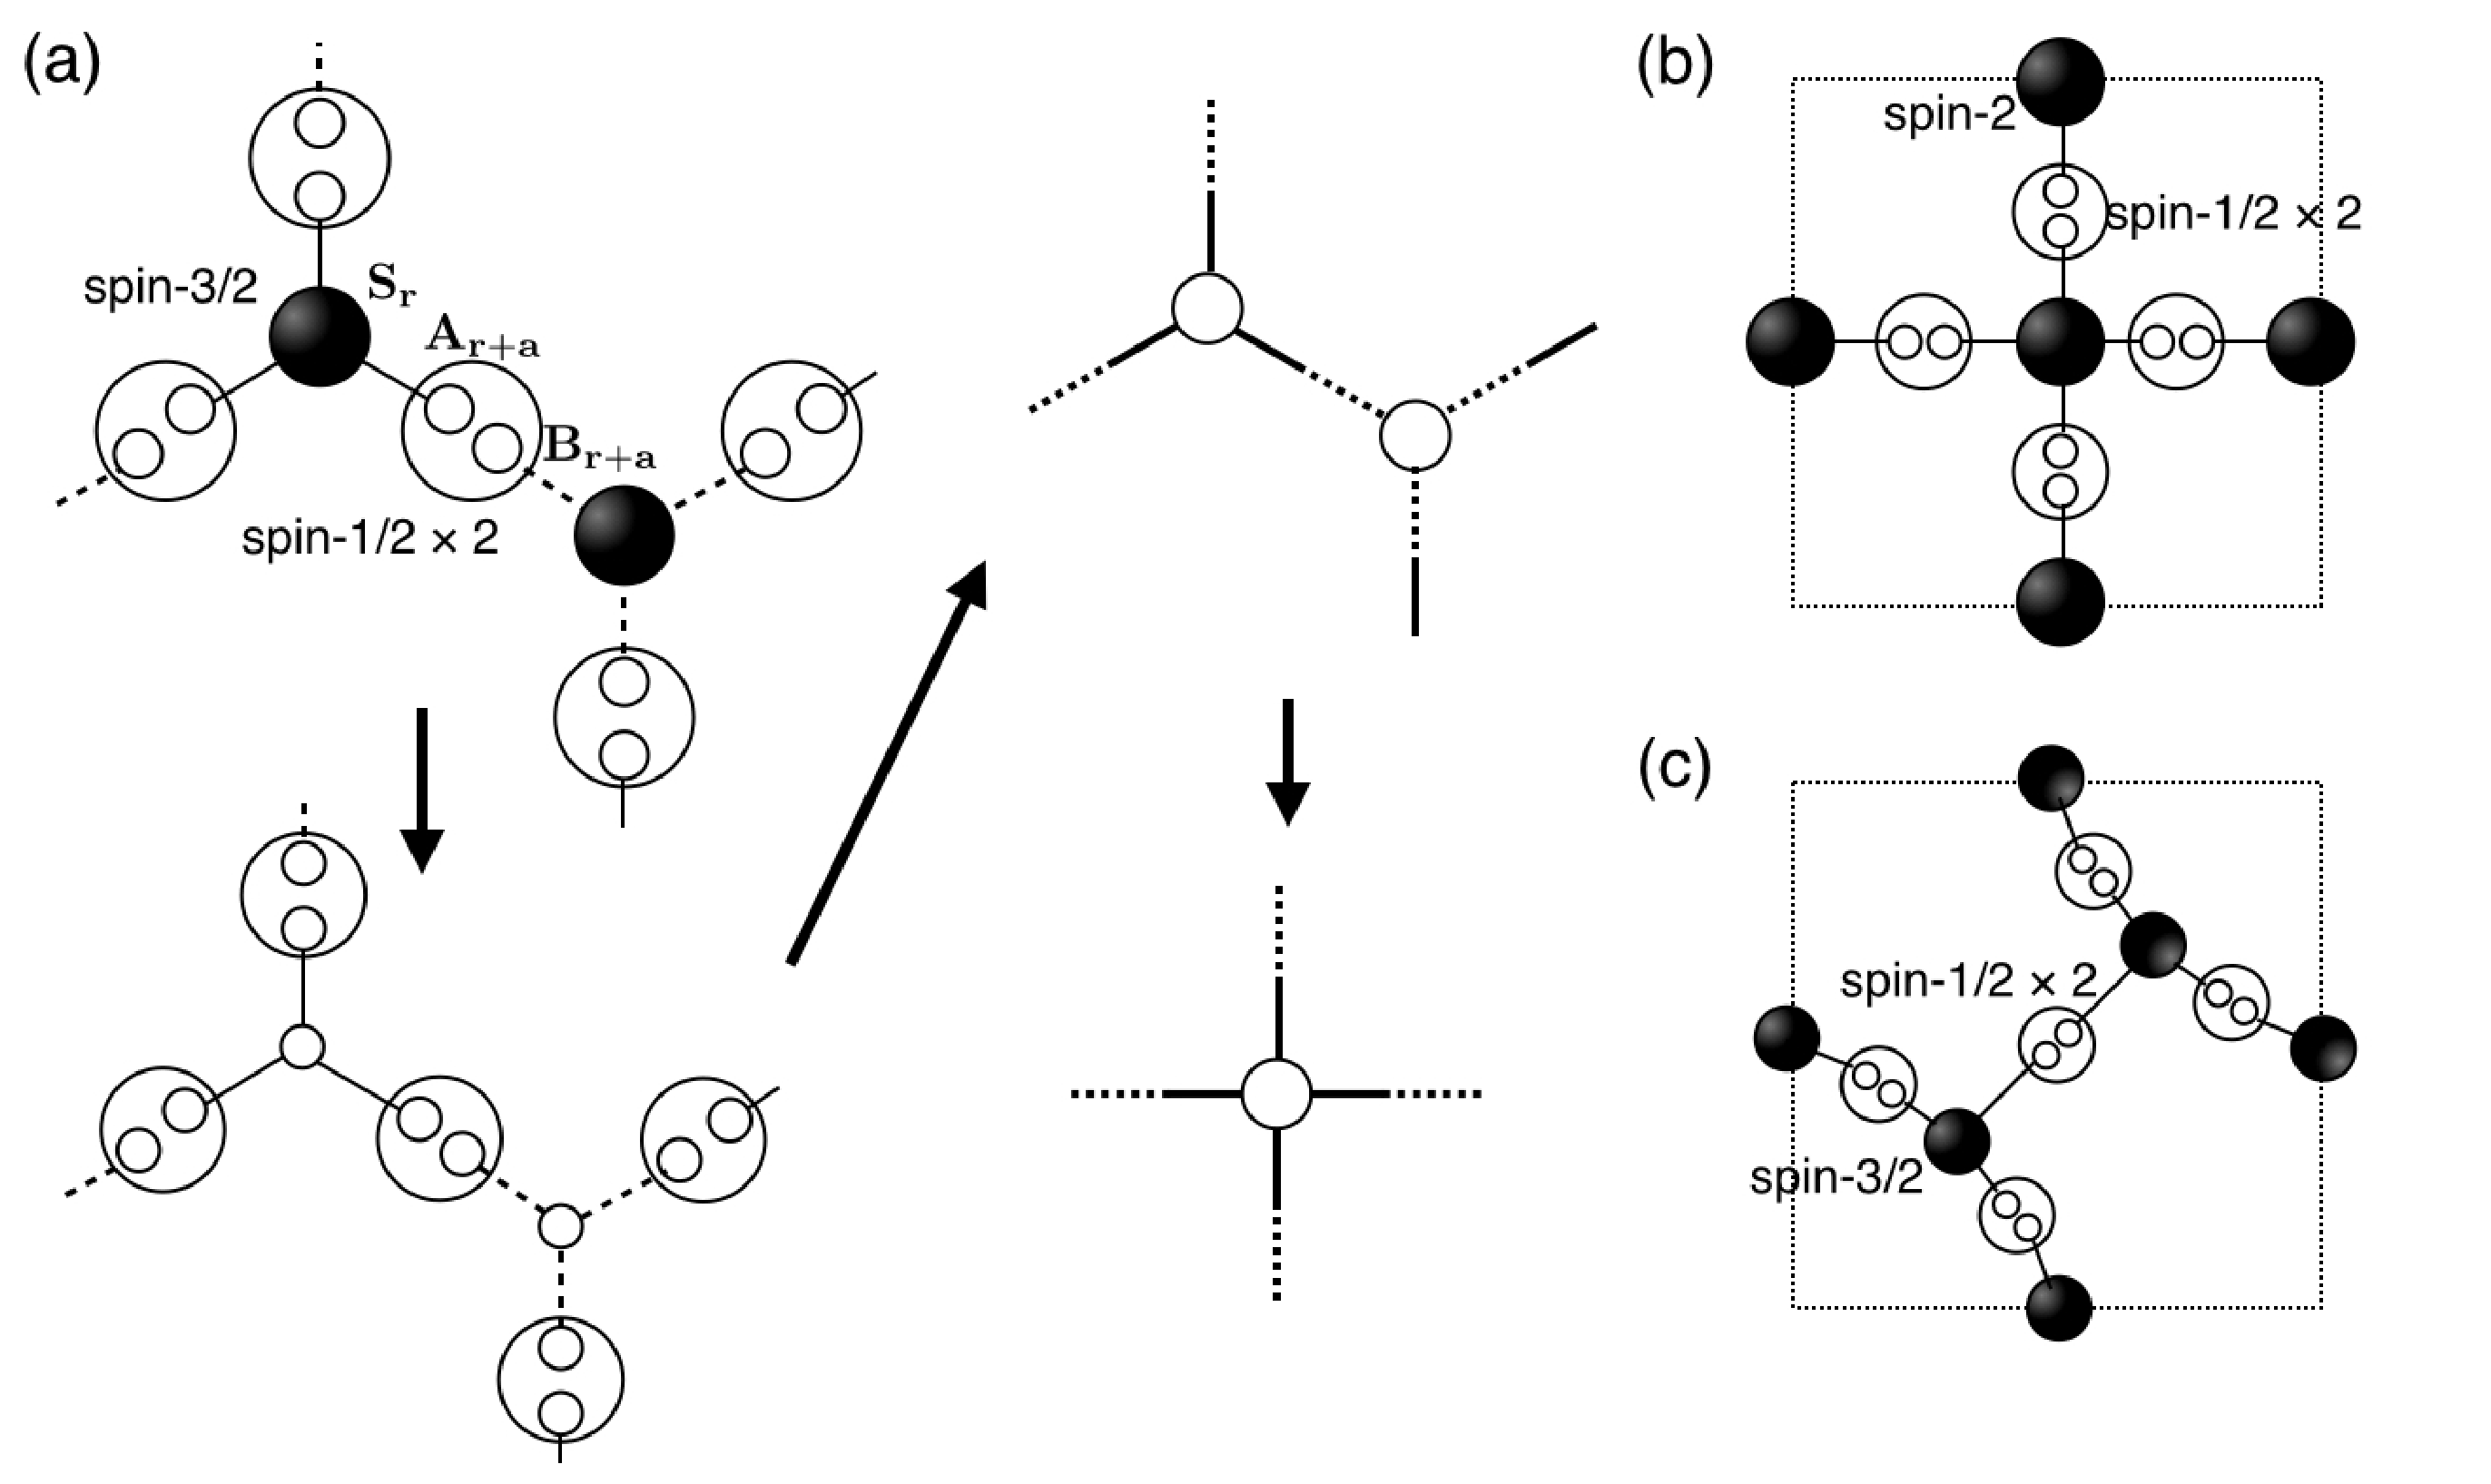
\includegraphics[width=130mm]{fig93.eps}
\caption{(a) A system consisting of spin-3/2 particles and composite particles of two spin-1/2.
After the filtering operation on the ground state, we obtain cluster states.
(b) A system consisting of spin-2 particles and composite particles of two spin-1/2 for the 3D cluster state.
(c) A system consisting of spin-3/2 particles and composite particles of two spin-1/2 for the 3D cluster state.
}
\label{fig93}
\end{figure}
%%%%

By using the threshold for topologically protected MBQC, we can calculate the threshold temperatures $T=0.21\Delta$ and $T=0.18\Delta$ for the cases of spin-2 and spin-3/2 center particles, respectively~\cite{LiKwek,FujiiMoriTher}.
Accordingly, we can perform 
fault-tolerant universal measurement-based quantum computation
even on the thermal states of local two-body Hamiltonians 
at finite temperature. 
